\chapter{BroodwarBotQ}%: putting it all together}
%%% There's no difference between a pessimist who says, "Oh it's hopeless, so don’t bother doing anything." and an optimist who says, "Don't bother doing anything, it's going to turn out fine anyways. Either way, nothing happens.
%%% --Yvon Chouinard
\label{chapter:bot}


%%% BBQ LOC
%%% cpp:          23234

\begin{quotation}
\textit{Dealing with failure is easy: Work hard to improve. Success is also easy to handled: You've solved the wrong problem. Work hard to improve.}\\
\begin{flushright}Alan J. Perlis (1982)\end{flushright}
\end{quotation}

\lettrine{I}{n} this chapter, we present some of the engineering that went in the robotic player (bot) implementation, which may help the comprehension of the organization and utility of the different chapters. We will also present the different flows of informations and how decisions are made during a game. Finally we will present the results of the full robotic player to various bots competitions.

\ifthenelse{\equal{\myebookformat}{false}}{
\chaptertoc
}{}


%\citep{Wolfe11} % BOUNDED INTENTION PLANNING TODO

\section{Code architecture}

\label{sec:codearchitecture}

Our implementation\footnote{\textsc{BroodwarBotQ}, code and releases: \url{http://github.com/SnippyHolloW/BroodwarBotQ}} (BSD licensed) uses BWAPI\footnote{BWAPI: \url{http://code.google.com/p/bwapi/}} to get information from and to control StarCraft. The bot's last major revision (January 2011) consists of 23,234 lines of \texttt{C++} code, making good use of \texttt{boost} libraries and BWTA (Brood War Terrain Analyzer). The learning of the parameters from the replays is done by separated programs, which serialize the probability tables and distribution parameters, later loaded by \textsc{BroodwarBotQ} each game.


The global (simplified) view of the whole bot's architecture is shown in Figure~\ref{fig:codearchitecture}. There are three main divisions: ``Macro'' (economical and production parts), ``Intelligence'' (everything information related) and ``Micro'' (military units control/actions). Units (workers, buildings, military units) control is granted through a centralized \texttt{Arbitrator} to ``Macro'' parts and Goals. This is a bidding system in which parts wanting a unit bid on it relatively to the importance of the task they will assign it. There may (should) be better systems but it works. We will now detail the parts which were explained in the previous three chapters.

\begin{figure}[h]
\begin{center}
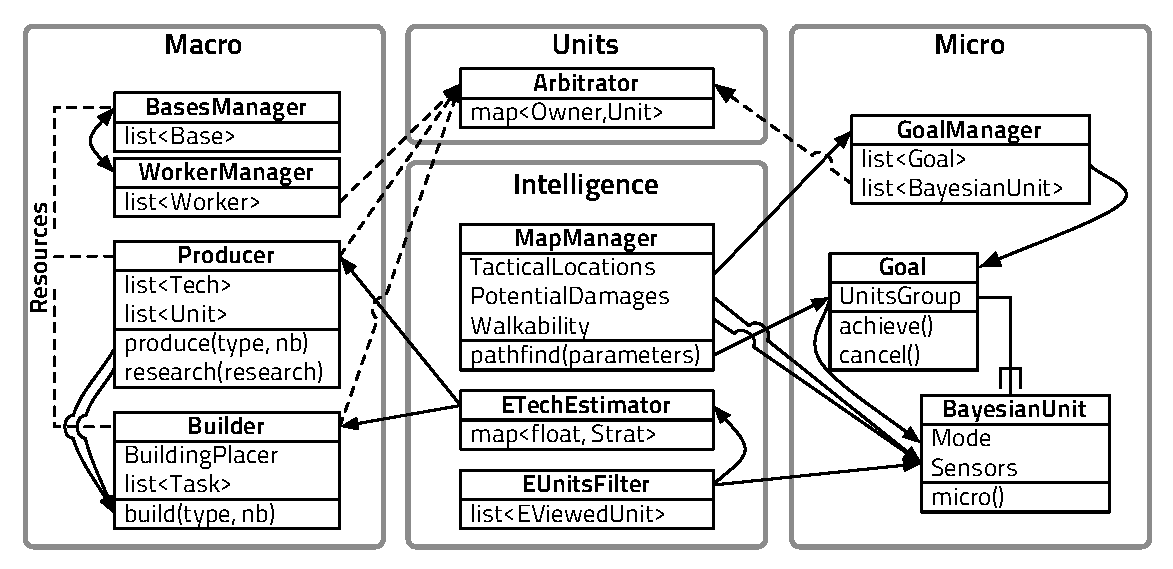
\includegraphics[width=16cm]{images/BBQEarly2012.pdf}
\caption{Simple view of the code architecture of \textsc{BroodwarBotQ}, the most important interactions are shown: every piece which has responsibility for the control of units refer to the \texttt{Arbitrator}, all macro components compete for resources, all other arrows represent orders or important transfers of information.}
\label{fig:codearchitecture}
\end{center}
\end{figure}
% mapping schéma code <-> schéma info-flow.

%We start by presenting short descriptions of the relative organizations of the different parts.

%%% \begin{figure}[h]
%%% \subsection{Micro-management}
%%% \begin{lstlisting}
%%% class UnitsGroup
%%% {
%%%     vector<BayesianUnit*> units;
%%%     vector<BayesianUnit*> arrivingUnits;
%%%     vector<Position> path;
%%%     virtual void update();
%%%     virtual void formation(Formation* f);
%%%     void takeControl(Unit* u);
%%%     void giveUpControl(Unit* u);
%%%     void switchMode(unit_mode um);
%%% };
%%% 
%%% void UnitsGroup::update()
%%% {
%%%     updateArrivingUnits();
%%%     updateCenter();
%%%     updateNearbyUnitsFromFilter();
%%%     chooseLeadingUnit();
%%%     if (groupMode == MODE_SCOUT || groupMode == MODE_MOVE)
%%%         temporaryPosition = groupTargetPosition;
%%%     if (mustFight()) // always false in MODE_SCOUT
%%%     {
%%%         if (outnumbered())
%%%             temporaryPosition = fallBackPosition;
%%%         else if (outnumbering())
%%%             temporaryPosition = groupTargetPosition;
%%%         else
%%%             temporaryPosition = NULL;
%%%     }
%%%     for each (BayesianUnit* bu in this->units)
%%%     {
%%%         bu->target = temporaryPosition;
%%%         bu->switchMode(selectMode());
%%%         bu->update();
%%%     }
%%% }
%%% \end{lstlisting}
%%% \caption{Simplified code listings for UnitsGroup}
%%% \label{fig:microcode1}
%%% \end{figure}
%%% 
%%% \begin{figure}[h]
%%% \begin{lstlisting}
%%% class BayesianUnit
%%% {
%%%     void setObjective(Position p);
%%%     virtual void update();
%%%     virtual void micro(); // fight
%%% };
%%% 
%%% class SpecialUnitType // an example of a specializing class
%%% {
%%%     void update();
%%%     void micro();
%%% };
%%% 
%%% 
%%% void BayesianUnit::micro() 
%%% {
%%%     updateRangeEnemies();
%%%     decideToFlee?();
%%%     if (iCanFire())
%%%     {
%%%         enemyTarget = selectTarget(); // uses the targetting heuristic
%%%         attackEnemyUnit(enemyTarget);
%%%     }
%%%     else if (lagControlOK)
%%%     {
%%%         if (iShouldFlee())
%%%             flee(); // updateDir with special attractors (damage gradient)
%%%         else
%%%             fightMove(); // updateDir with special attractors (priority target)
%%%     }
%%% }
%%% 
%%% void BayesianUnit::updateDir()
%%% {
%%%     updateAttractors(); // all the sensory inputs except the Objective
%%%     updateObj(); // Objective coming from the UnitsGroup
%%%     computeProbs(); // Bayesian fusion
%%%     selectDir(); // sampling in the possible directions if group > limit size
%%%     clickDir(); // performs the action
%%% }
%%% 
%%% void BayesianUnit::update()
%%% {
%%%     if (mode == MODE_FIGHT)
%%%         micro();
%%%     else
%%%         updateDir();
%%% }
%%% \end{lstlisting}
%%% \caption{Simplified code listings for BayesianUnit(s)}
%%% \label{fig:microcode2}
%%% \end{figure}

\subsection{Units control}
\label{sec:micromanagementcode}

As presented in chapter~\ref{chapter:micro}, units are controlled in a sensory-motor fashion through Bayesian fusion of physical or abstract influences. Units pursuing a common objective are regrouped in a \texttt{UnitsGroup}, which sets this objective for every unit it commands. This objective is generated for each unit from the needs of a higher-up \texttt{Goal} (see below) through \texttt{achieve()} or \texttt{cancel()}.

The \texttt{BayesianUnit} class has different fusion modes (see section~\ref{sec:unitsgroup}) set by the \texttt{UnitsGroup} depending on the \texttt{Goal} type and on the situation (number and types of enemies, terrain...). Its sensory inputs are fed by the \texttt{UnitsGroup} (objectives) and by the \texttt{MapManager} (potential damages, terrain) and the \texttt{EUnitsFilter} (enemy units).

A derivative (child) of the \texttt{BayesianUnit} class is instantiated for each unit that is controlled. A \texttt{BayesianUnit} is a modal \glos{FSM} as shown in Figure~\ref{fig:unit_HFSM}. It presents a simple interface to move and fight (the \texttt{micro()} method). Some parameter can be specialized depending on the particularities of unit types:
\begin{itemize}
    \item the list of priority unit types to target (because of units attacks efficiencies as in rock/paper/scissors),
    \item the reasons for which to flee (\texttt{flee?()}),
    \item \texttt{micro()} itself can be specialized further if the two points above do not suffice to produce a skillful behavior (for very special unit types: casters).
\end{itemize}
A call to \texttt{micro()} then decides of the course of actions during a fight (applying Bayesian fusion with the right sensory inputs when moving).


\subsection{Tactical goals}
\label{sec:goals}
The decision that we want our AI system to make at this level is \textit{where} and \textit{how} to attack. This is reflected in the StarCraft bot as a \texttt{Goal} creation. \texttt{Goals} are interfacing high level tactical thinking with the steps necessary to their realization. A \texttt{Goal} recruits units and binds them under a \texttt{UnitsGroup} (see section~\ref{sec:unitsgroup}). A \texttt{Goal} is an \glos{FSM} in which two states are simple planners (an FSM with some form of procedural autonomy), it has:
\begin{itemize}
    \item preconditions, for instance a \textit{drop} attack needs to specify at least a transport unit (Shuttle/Dropship/Overlord) and ground attack units.
    \item hard states: \textit{waiting precondition, in progress, in cancel, achieved, canceled}, which corresponds to the \texttt{Goal} advancement..
    \item \textit{and} and/or \textit{or} logic subgoals with:
        \begin{itemize}
            \item a realization test
            \item a proposition of action to try to realize it
            \item an estimation of the ``distance'' to realization
        \end{itemize}
\end{itemize}
In the \textit{in progress} and \textit{in cancel} modes, the ``plan'' is a simple search in the achievable subgoals and their ``distance'' to realization.

The tactical model can specify \textit{where} to attack by setting a localized subgoal (Formation/See/Regroup/KillSubgoal...) to the right place. It can specify \textit{how} by setting the adequate precondition(s). It also specifies the priority of a \texttt{Goal} so that it has can bid on the control of units relatively to its importance. The \texttt{GoalManager} updates all \texttt{Goals} that were inputed and act as a proxy to the \texttt{Arbitrator} for them.

\subsection{Map and movements}

The \texttt{MapManager} keeps track of:
\begin{itemize}
    \item the economical and military bases (positions) of the enemy, 
    \item the potential damages map, which is updated with each new observations (units, spells...),
    \item the ``walkability'' of the terrain (static terrain and buildings).
\end{itemize}
It also provides threaded pathfinder services which are used by \texttt{UnitsGroup}s to generate objectives waypoints when the \texttt{Goal}'s objectives are far. This pathfinder can be asked specifically to avoid certain zones or tiles.

\subsection{Technology estimation}

The \texttt{ETechEstimator} does constant \glos{buildtree} prediction as explained in section~\ref{sec:techtreepred}, and so it exposes the distribution on the enemy's \glos{techtree} as a ``state estimation service'' to other parts of the bot taking building and production decision. It also performs \gloss{opening} prediction during the first 15 minutes of the game, as explained in section~\ref{sec:openingspred}. 

New enemy units observations are taken into account instantly. When we see an enemy unit at time $t$, we infer that all the prerequisites were built at least some time $t'$ earlier according to the formula:
$t' = t - ubd - umd$
with $ubd$ being the unit's building duration (depending on the unit type), and $umd$ being the unit's movement duration depending on the speed of the unit's type, and the length of the path from its current position to the enemy's base. We can also observe the upgrades that the units have when we see them, and so we take that into account the same way. For instance, if a unit has an attack upgrade, it means that the player has the require building since at least the time of observation minus the duration of the upgrade research.

The distribution on \gloss{opening} computed by the \texttt{ETechEstimator} serves the purpose of recognizing the short term intent of the enemy. This way, the \texttt{ETechEstimator} can suggest the production of counter measures to the opponent's strategy and special tactics. For instance, when the belief that the enemy is doing a ``Dark Templars'' opening (an opening aimed at rushing invisible technology before the time at which a standard opening reaches detector technology, to inflict massive damage) pass above a threshold, the \texttt{ETechEstimator} suggests the construction of turrets (Photon Cannon, static defense detectors) and Observers (mobile detectors).

\subsection{Enemy units filtering}

At the moment, enemy units filtering is very simple and just diffuse uniformly (with respect to its speed) the probability of a unit to be where it was last seen before totally forgetting about its position (not its existence) when it was not seen for too long. We will now shortly present an improvement to this enemy units tracking.

\subsubsection{A possible improved enemy units tracking/filtering}

\label{sec:enemyunitsfilter}
We consider a simple model, without speed nor steering nor $See$ variable for each position/unit. The fact that we see positions where the enemy units are is taken into account during the update.
The idea is to have (learn) a multiple influences transition matrix on a Markov chain on top of the regions discretization (see chapter~\ref{chapter:tactics}), which can be seen as one Markov chain for each combination of motion-influencing factors.

The \textbf{perception} of such a model would be for each unit if it is in a given region, as the bottom diagram in Figure~\ref{fig:BWTA}. From there, we can consider either map-dependent regions, regions uniquely identified as they are in given maps that is; or we can consider regions labeled by their utility. We prefer (and will explain) this second approach as it allows our model to be applied on unknown (never seen) maps directly and allows us to incorporate more training data. The regions get a number in the order in which they appear after the main base of the player (e.g. see region numbering in Fig.~\ref{fig:terrainanalysis} and~\ref{fig:examplefilter}). %For instance regions ordering is $1 \rightarrow main\_base, 2 \rightarrow first\_expansion, 3 \rightarrow

\vspace{0.3cm}
\textit{Variables}\\
%There are $p$ regions, the full filter works on $m$ units, each of the units is represented by $n$ particles.
The full filter works on $n$ units, each of the units having a mass in the each of the $m$ regions.

%%% \begin{itemize}
%%%     \item $Agg \in \{T,F\}$, the player's aggressiveness (is he attacking or defending?), which can comes from other models but can also be an output here. 
%%%     \item $UT_{i \in \llbracket 1\dots m \rrbracket} \in \{unit\ types\}$ the type of the $i$th tracked unit.
%%%     \item $X^{t-1}_{i \in \llbracket 1\dots m \rrbracket , j \in \llbracket 1\dots n \rrbracket} \in \{regions\}\ i.e.\ \in \llbracket 1 \dots p \rrbracket$ the $j$th particle for the $i$th unit at time $t-1$.
%%%     \item $X^{t}_{i \in \llbracket 1\dots m \rrbracket , j \in \llbracket 1\dots n \rrbracket} \in \{regions\}$, the $j$th particle for the $i$th unit at time $t$.
%%% \end{itemize}
\begin{itemize}
    \item $Agg \in \{true,false\}$, the player's aggressiveness (are they attacking or defending?), which can comes from other models but can also be an output here. 
    \item $UT_{i \in \llbracket 1\dots n \rrbracket} \in \{unit\ types\}$ the type of the $i$th tracked unit, with $K$ unit types.
    \item $X^{t-1}_{i \in \llbracket 1\dots n \rrbracket} \in \llbracket r_1 \dots r_m \rrbracket$, the region in which is the $i$th unit at time $t-1$.
    \item $X^{t}_{i \in \llbracket 1\dots n \rrbracket} \in \llbracket r_1 \dots r_m \rrbracket$, the region in which is the $i$th unit at time $t$.
\end{itemize}

%we have And the $Map \in \{maps\}$ variable for map dependent models. 

\vspace{0.3cm}
\textit{Joint Distribution}\\
We consider all units conditionally independent give learned parameters. (This may be too strong an assumption.) %(false, we could cluster armies: but we can hope the parameters will account for units traditionally moving together).\\

%%% \begin{eqnarray}
%%% & & \PP(Agg, UT_{1:m}, X^{t-1,t}_{1:m,1:n}) \\
%%% & = & \PP(Agg)\prod_{i=1}{m} \PP(UT_{i}\\
%%% & \times & \prod_{j=1}{n} \PP(X^{t-1}_{i,j} \PP(X^t_{i,j}|X^{t-1}_{i,1:n},UT_i,Agg)
%%% \end{eqnarray}
\begin{eqnarray}
& & \PP(Agg, UT_{1:m}, X^{t-1,t}_{1:m,1:n}) \\
& = & \PP(Agg)\prod_{i=1}^{n} \left[ \PP(UT_{i}) \PP(X^{t-1}_{i}) \PP(X^t_{i}|X^{t-1}_{i},UT_i,Agg)\right]
\end{eqnarray}

\vspace{0.3cm}
\textit{Forms}\\

\begin{itemize}
    \item $\PP(Agg)=Binomial(p_{agg})$ is a binomial distribution.
    \item $\PP(UT_i)=Categorical(K,p_{ut})$ is categorical distribution (on unit types).
    \item $\PP(X^{t-1}_{i})=Categorical(m, p_{reg})$ is a categorical distribution (on regions).
    \item $\PP(X^t_i|X^{t-1}_i,UT_i,Agg)$ are $\#\{units\_types\} \times \abs{Agg} = K \times 2$ different $m\times m$ matrices of transitions from regions to other regions depending on the type of unit $i$ and of the aggressiveness of the player. (We just have around 15 unit types per race ($K \approx 15$) so we have $\approx 15\times 2$ different matrices for each race.)
\end{itemize}


\vspace{0.3cm}
\textit{Identification (learning)}\\

$\PP(X^t_i|X^{t-1}_i, UT_i, Agg)$ is learned with a Laplace rule of succession from previous games. Against a given player and/or on a given map, one can use $\PP(X^t_i|X^{t-1}_i, UT_i, Agg, Player, Map)$ and use the learned transitions matrices as priors. When a player attacks in the dataset, we can infer she was aggressive at the beginning of the movements of the army which attacked. When a player gets attacked, we can infer she was defensive at the beginning of the movements of the army which defended. At other times, $\PP(Agg=true) = \PP(Agg=false) = 0.5$.
\begin{eqnarray*}
& & PP(X^t_i=r|X^{t-1}_i=r', UT_i=ut, Agg=agg) \\
& \propto & \frac{1+n_{transitions}(r'\rightarrow r, ut, agg)\PP(agg)}{\#\{entries\_to\_r\} + \sum_{j=1}^{m} n_{transitions}(r' \rightarrow r_j, ut, agg)\PP(agg)}
\end{eqnarray*}

Note that we can also (try to) learn specific parameters of this model during games (not a replay, so without full information) against a given opponent with \glos{EM} to reconstruct and learn from the most likely state given all the partial observations.

\vspace{0.3cm}
\textit{Update (filtering)}\\

\begin{itemize}
    \item When a unit $i$ becomes hidden, which was seen in region $r$ just before, we have:
\begin{eqnarray*}
\begin{cases}
\PP(X^t_{i} = r) = 1.0\\
\PP(X^t_{i} = r_j) = 0.0\ \forall j \ \mathrm{iff}\ r_j \neq r
\end{cases}
\end{eqnarray*}

    \item For all regions $r$ that we see ``totally'' (above a threshold of a percentage of the total area), we set $\PP(X^t_i = r) = 0.0$ and redistribute their probability mass to hidden (or still partially hidden) regions (algorithm~\ref{alg:cullingfilter}):
\begin{algorithm}[!h]
\caption{Culling/updating algorithm for filtering visible regions}
\label{alg:cullingfilter}
\begin{algorithmic}
\ForAll{$i \in \{enemy\_units\}$}
    \State $s \leftarrow 0.0$
    \ForAll{$r \in \{visible\_regions\}$}
        \State $s \leftarrow s + \PP(X^{t-1}_i = r)$
        \State $\PP(X^{t-1}_i = r) = 0.0$
    \EndFor
    \State $total \leftarrow \sum_{j=1}^m \PP(X^{t-1}_i=r_j)$
    %\State $k \leftarrow \#\{\neg visible\_regions\}$
    \ForAll{$r \in \{\neg visible\_regions\}$}
        \State $\PP(X^t_i = r) \leftarrow \PP(X^t_i = r) + \frac{s}{total}\times \PP(X^{t-1}_i = r)$
    \EndFor
\EndFor
\end{algorithmic}
\end{algorithm}

    \item For all the other cases, we have:
$$\PP(X^t_{i} = r) = \sum_{j=1}^{m} \PP(X^{t-1}_i = r_j')\PP(X^t_i = r | X^{t-1}_i = r_j', UT_i, Agg)$$
\end{itemize}

\vspace{0.3cm}
\textit{Questions}\\

\begin{itemize}
    \item When we want to infer where the $n$ enemy units are, we ask:
\begin{eqnarray*}
& & \PP(X_{1:n}^t| UT_{1:n}=ut_{1:n})\\
& \propto & \sum_{Agg} \PP(Agg) \prod_{i=1}^n \PP(ut_i) \sum_{X_i^{t-1}} \PP(X_i^t|X_i^{t-1},ut_i,Agg)\\
& \propto & \sum_{Agg=false}^{true} \PP(Agg) \prod_{i=1}^n \PP(UT_i=ut_i) \sum_{j = 1}^{m} \PP(X_i^t|X_i^{t-1}=r_j,ut_i,Agg)
\end{eqnarray*}
    \item When we want to infer the aggressiveness of the enemy (from the troupes' movements that we have seen), we ask:
\begin{eqnarray*}
& & P(Agg | UT_{1:n} = ut_{1:n})\\
& \propto & \PP(Agg) \prod_{i=1}^{n} \PP(ut_i)\sum_{X_i^{t-1}}\PP(X_i^{t-1}) \sum_{X_i^{t}}  \PP(X_i^t|X_i^{t-1},ut_i,Agg) 
\end{eqnarray*}
\end{itemize}

\vspace{0.3cm}
\textit{Conclusion}\\
\vspace{0.3cm}

Offline learning of matrices (as shown in Fig.~\ref{fig:examplefilter}) of aggressive and defensive probable region transitions (for a given unit type). With online learning (taking previous offline learned parameters as priors), we could learn preferences of a given opponent.

\begin{figure}
\begin{center}
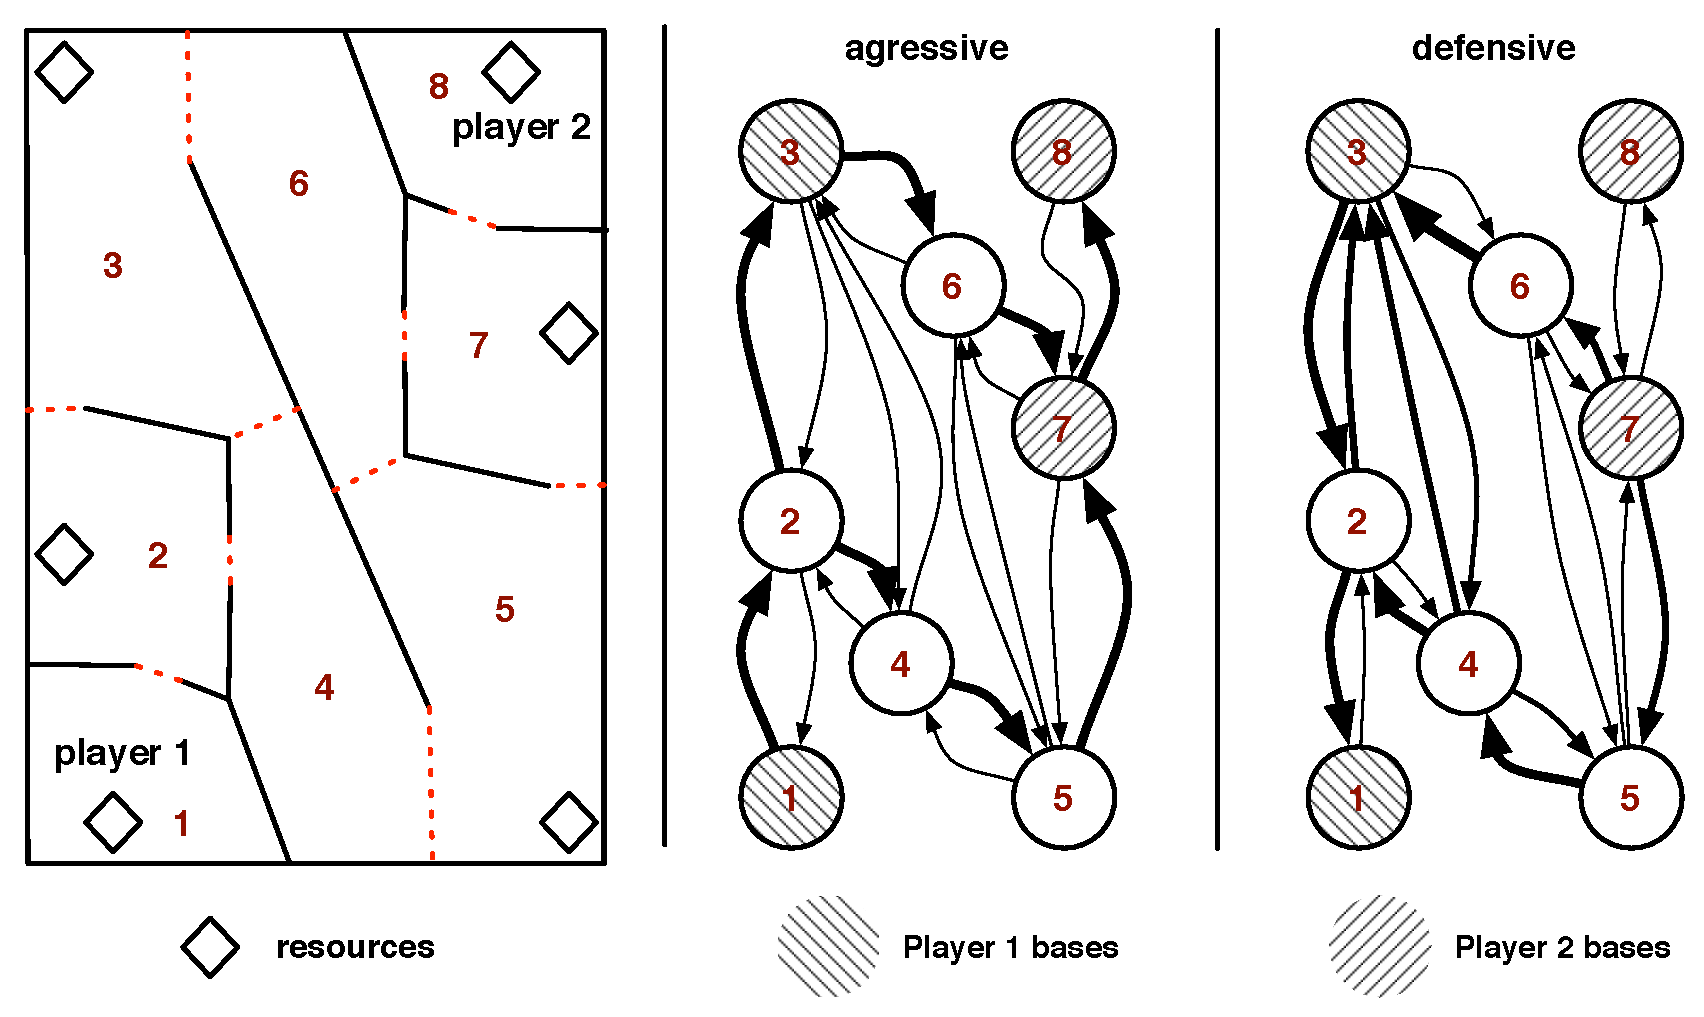
\includegraphics[width=15cm]{images/units_filter_markov.pdf}
\caption{Example of the units filter transition matrices on a simple map (same as in Fig.~\ref{fig:terrainanalysis}) for aggressive and defensive sets of parameters for a given unit type. The thickness of the arrows is proportional to the transition probability between regions.}
\label{fig:examplefilter}
\end{center}
\end{figure}

By considering a particle filter \citep{Thrun02d}, we could consider a finer model in which we deal with positions of units (in pixels or walk tiles or build tiles) directly, but there are some drawbacks:
\begin{itemize}
    \item The data to learn (offline or online) is sparse as there are several versions of the same map and the combinatorics of start positions (2 occupied start positions on 4 possible most of the time). This would need any form of spatial abstraction anyway, like distance to most walked traces.
    \item Computation cost to track $\approx 40$ units makes it so that the particle sampling numbers should be low to stay real-time. Or that one should abandon the motion model for a Kalman filter \citep{Kalman1960}. 
\end{itemize}
The advantages are not so strong: 
\begin{itemize}
    \item (hopefully) more precision in units position estimation,
    \item possibilities to have more complex motion models (updates/culling of the filter),
    \item differentiation between trajectories of ground and flying units,
    \item differentiation between different trajectories of attacks inside large regions.
\end{itemize}
We would like to implement our regions-based enemy units filtering in the future, mainly for more accurate and earlier tactical prediction (perhaps even drop tactics interception) and better tactical decision making.

%\clearpage

\section{A game walk-through}

We will now show key moments of the game, as was done with a human-played game in section~\ref{sec:astarcraftgame}, but from the bot's point of view (with debug output).

\begin{figure}[h]
\begin{center}
\begin{tabular}{cc}
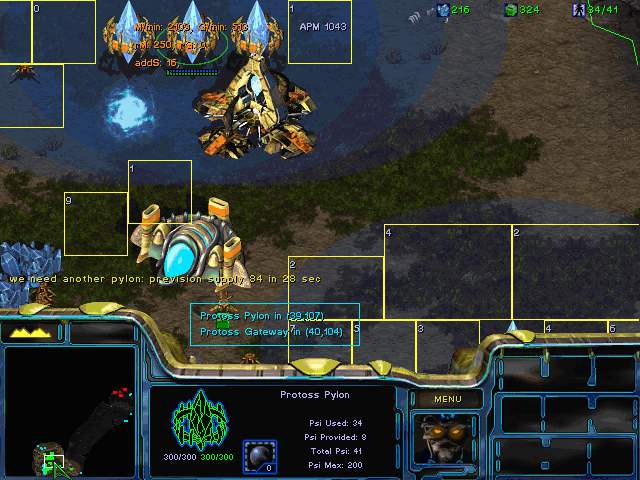
\includegraphics[width=0.90\columnwidth]{images/botgame/macro0.png}
\end{tabular}
\caption{A full screen capture of some debug output of economical parts of BroodwarBotQ. The orange text at the top left shows the minerals/minute and gas/minute rates as well as the resources reserved for planned buildings and additional supply. The teal (light blue) rectangle at the bottom of the game's view shows the buildings that will be constructed (and their future tentative positions). The big transparent (translucent) blue ellipses show the Pylons construction coverage. The yellow rectangles (with numbers in their top left corners) show the future buildings planned positions.}
\label{fig:bot_macro}
\end{center}
\end{figure}

First, Figure~\ref{fig:bot_macro} shows some economical elements of BBQ. The yellow rectangles show future buildings placements. In the light blue (teal color) rectangle are the next buildings which are planned for construction with their future positions. Here, the Protoss Pylon was just added to the construction plan as our \texttt{Producer} estimated that we will be \glos{supply} blocked in 28 seconds at the current production rate. This is noted by the ``we need another pylon: prevision supply 84 in 28 sec'' line, as supply is shown doubled (for programmatic reasons, so that supply is always an integer): 84 is 42, and we have a current \glos{maxsupply} of 41 (top right corner). 

Our buildings placer make it sure that there is always a path around our buildings blocks with a flow algorithm presented in the appendix in algorithm~\ref{alg:flood} and Figure~\ref{fig:buildingsplacer}. It is particularly important to be able to circulated in the base, and that newly produced units are not stuck when they are produced (as they could is there was a convex enclosure as in Fig.~\ref{fig:buildingsplacer}). Buildings cannot be placed anywhere on the map, even more so for Protoss buildings, as most of them need to be build under Pylon coverage (the plain blue ellipses in the screenshot). At the same time, there are some (hard) tactical requirements for the placement of defensive buildings\footnote{A good benchmark for buildings positioning would be to test if an AI can perform a ``Forge expand'' which consists in blocking all ground paths with buildings and protecting against the early rushes with judiciously placed Photon Cannons, without any military unit.}. 

\begin{figure}[h]
\begin{center}
\begin{tabular}{c}
%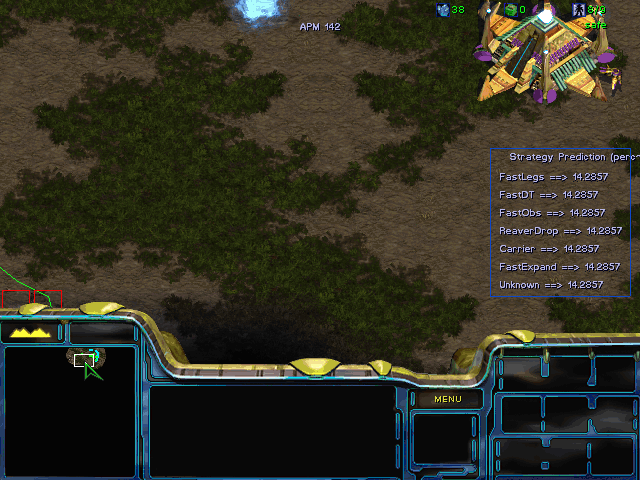
\includegraphics[width=0.49\columnwidth]{images/botgame/scout0.png} &
%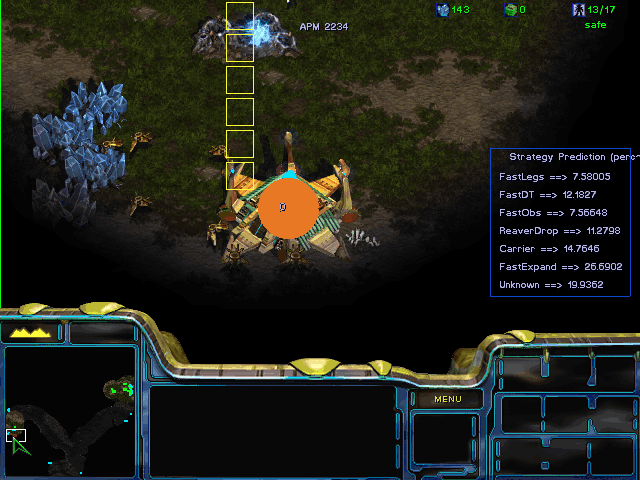
\includegraphics[width=0.49\columnwidth]{images/botgame/scout0b.png} \\
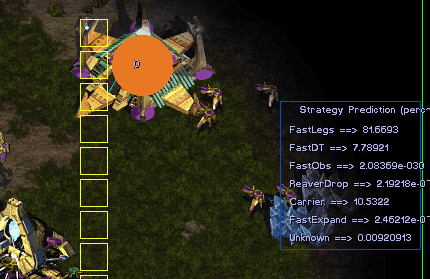
\includegraphics[width=0.66\columnwidth]{images/botgame/scout1.png}\\
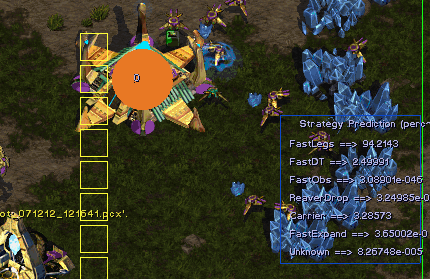
\includegraphics[width=0.66\columnwidth]{images/botgame/scout2.png}
\end{tabular}
\caption{Crops of screenshots of the first scouting (discovery) of an opponent's base in a Protoss vs Protoss game. The buildings shown here are the ones of the opponent. The yellow squares represent the pathfinding output. On the bottom, in the blue rectangle, are displayed the possible openings for the Protoss opponent and their respective probabilities (in percentage) according what we have seen. The top picture was captured a few seconds before the right one and thus we had less information about the opponent's buildings (the upper right part is black because of the fog of war).}
\label{fig:bot_scout}
\end{center}
\end{figure}

At the beginning of the game, we have no idea about what the opponent is doing and thus our belief about their opening equals the prior (here, we set the priori to be uniform, see section~\ref{sec:openingspossibleimprovements} for how we could set it otherwise) we send a worker unit to ``scout'' the enemy's base both to know where it is and what the enemy is up to. Figure~\ref{fig:bot_scout} shows when we first arrive at the opponent's base in a case in which we have a strong evidence of what the opponent is doing and so our beliefs are heavily favoring the ``Fast Legs'' opening (in the blue rectangle on the right). We can see that with more information (the bottom picture) we make an even stronger prediction.

\begin{figure}[h]
\begin{center}
%\begin{tabular}{cc}
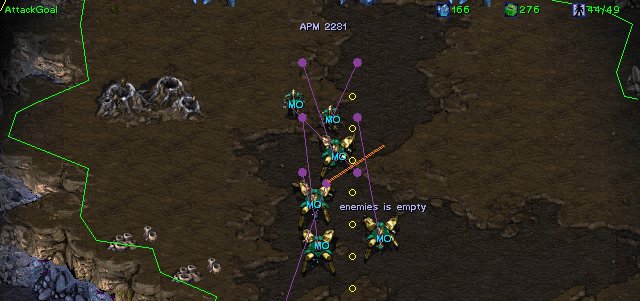
\includegraphics[width=0.69\columnwidth]{images/botgame/attack0.png}
\vspace{0.12cm}\\
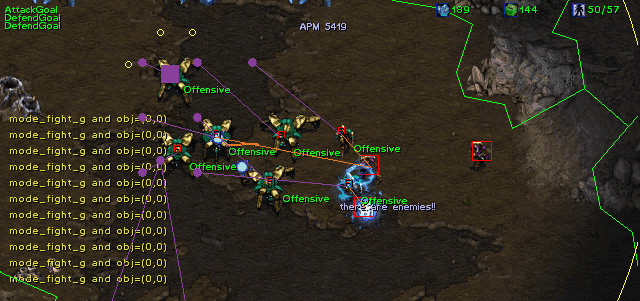
\includegraphics[width=0.69\columnwidth]{images/botgame/attack1.png}
\vspace{0.12cm}\\
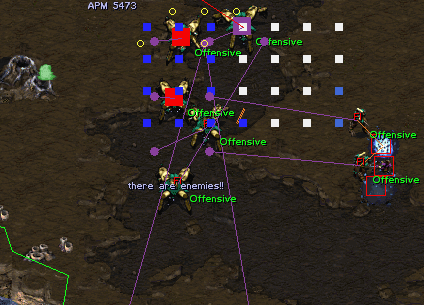
\includegraphics[width=0.496\columnwidth]{images/botgame/attack2.png}
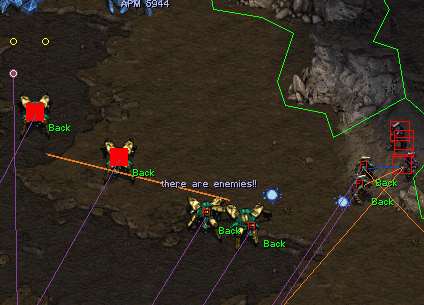
\includegraphics[width=0.496\columnwidth]{images/botgame/attack3.png}
%\end{tabular}
\caption{Crops of screenshots of an attack towards a Protoss opponent. The first screenshot (top) shows the units arriving at their formation \texttt{SubGoal} objectives (purple disks), the second shows the switch to the fight mode (for ground units) with the first enemy units appearing on the right. The third (bottom left) and fourth (bottom right) screenshots show the battle as it happens. The small squares (white to blue) show the attraction of one unit for its possible directions ($\PP(Dir_i) \forall i$): the whiter it is, the higher the probability to go there.}
\label{fig:bot_attack}
\end{center}
\end{figure}

If our bot does not have to defend an early rush by the opponent, it chooses to do a ``push'' (a powerful attack towards the front of the opponent's base) once it has a sufficient amount of military units, while it \gloss{expand} (take a second base) or opens up its \glos{techtree}. The first push is depicted in Figure~\ref{fig:bot_attack}: 
\begin{itemize}
    \item First (top), we regroup our forces in front of the opponent's base with a formation \texttt{SubGoal}.
    \item By trying to enter the opponent's base (second screenshot), our units have to fight they way through.
    \item The bottom left picture shows the distribution on $\PP(Dir_i)$ for the possible movements directions of one of the units at the top. We can see that it wants to avoid collision with allied units while going towards its target.
    \item The bottom right picture shows our units ``kiting back'' (retreating while fighting) to avoid being exposed in the ramp up the cliff (right part of the image).
\end{itemize}
BroodwarBotQ then goes up the ramp and destroys the base of the built-in AI.

\clearpage

\section{Results}

BroodwarBotQ (BBQ) consistently beats the built-in StarCraft: Broodwar AI\footnote{The only losses that our bot suffers against the built-in AI are against Zerg when the built-in AI does a quick zergling rush attack (``6 pool'') on small maps. Human players who successfully counter this have a good micro-management of workers as well as an efficient replanning of the first buildings (which is not BBQ's case).}, to a point that the original built-in AI is only used to test the stability of our bot, but not as a sparing/training partner.

BroodwarBotQ took part in the Artificial Intelligence and Interactive Digital Entertainment (AAAI AIIDE) 2011 StarCraft AI competition. It got 67 games counted as ``crashes'' on 360 games because of a misinterpretation of rules on the first frame\footnote{the additional terrain analysis was not serialized and taking more than one minute on the frame 0, which has no special tolerance as opposed as the year before.}, which is not the real unstability of the bot ($\approx$ 0,75\% as seen in \ref{fig:ladderbots}). The results of AIIDE are in Table~\ref{tab:botsAIIDE}.

\begin{table}[h]
    \begin{center}
    \begin{scriptsize}
    \begin{tabular}{|l|l|l|c|l|}
        \hline
        bot & race & refs & win rate & notes \\
        \hline
     Skynet%\footnote{\url{http://code.google.com/p/skynetbot/} } 
& Protoss & & 0.889 & openings depending on opponent's race \\
UAlbertaBot & Protoss & \citep{Churchill2011} & 0.794 & always 2-Gates opening \\
       Aiur%\footnote{\url{http://code.google.com/p/aiurproject/}} 
& Protoss & & 0.703 & robust and stochastic strategies \\
ItayUndermind & Zerg & & 0.658 & 6-pooling \\
       EISBot%\footnote{\url{http://code.google.com/p/eisbot/}} 
& Protoss & \citep{WeberCIG10,Weber2010cr} & 0.606 & 2-Gates or Dragoons opening \\
         SPAR%\footnote{\url{http://www.planiart.usherbrooke.ca/projects/spar/}} 
& Protoss & \citep{Kabanza2010} & 0.539 & uses Dark Templars \\
    Undermind & Terran & & 0.517 & Barracks units \\
         Nova%\footnote{\url{http://www.planiart.usherbrooke.ca/projects/spar/}} 
& Terran & \citep{NovaBot2011} &  0.475 & robust play \\
 BroodwarBotQ%\footnote{\url{https://github.com/SnippyHolloW/BroodwarBotQ}} 
& Protoss  & %\citep{SYNNAEVE:OpeningPred} \citep{SYNNAEVE:Micro} 
& 0.328 & adapts to the opening \\
        BTHAI%\footnote{\url{http://code.google.com/p/bthai/}} 
& Zerg & \citep{Hagelback2009} & 0.319 & Lurkers opening  \\
    Cromulent & Terran & & 0.300 & Factory units \\
   bigbrother & Zerg & & 0.278 & Hydralisks and Lurkers \\
       Quorum & Terran & & 0.094 & expands and produce Factory units \\
        \hline
    \end{tabular}
    \end{scriptsize}
    \end{center}
    \caption{Result table for the AIIDE 2011 StarCraft AI competition with 360 games played by each bot.}
    \label{tab:botsAIIDE}
\end{table}
%%% AIIDE 2011
%%% Skynet
%%% UAlbertaBot
%%% Aiur
%%% ItayUndermind
%%% EISBot
%%% SPAR
%%% Undermind
%%% Nova
%%% BroodwarBotQ
%%% BTHAI
%%% Cromulent
%%% bigbrother
%%% Quorum

Also in 2011 was the Computational Intelligence and Games (IEEE CIG) 2011 StarCraft AI competition. This competition had 10 entries\footnote{BroodwarBotQ \url{https://github.com/SnippyHolloW/BroodwarBotQ}, BTHAI \url{http://code.google.com/p/bthai/}, AIUR \url{http://code.google.com/p/aiurproject/}, LSAI \url{http://cs.lafayette.edu/~taylorm}, 
EvoBot, Protoss Beast Jelly \url{http://wwbwai.sourceforge.net/}, Xelnaga (modified AIUR), Skynet \url{http://code.google.com/p/skynetbot/}, Nova \url{http://nova.wolfwork.com/}, UAlbertaBot} and BroodwarBotQ placed 4th with a little luck of seed (it did not have to play against Aiur). The finals are depicted in Table~\ref{tab:botsCIG}.
\begin{table}[h]
    \begin{center}
    \begin{tabular}{|l|c|c|c|c|}
        \hline
bot & race & crashes & games & wins \\ 
        \hline
Skynet & Protoss & 0 & 30 & 26 \\ 
UAlbertaBot & Protoss & 0 & 30 &  22\\
Xelnaga\footnote{A modified version of AIUR doing only Dark Templar rushes.} & Protoss & 3 & 30 & 11 \\
BroodwarBotQ & Protoss & 2 & 30 & 1\\
        \hline
    \end{tabular}
    \end{center}
    \caption{Result table of the finals for the CIG 2011 StarCraft AI competition (10 entries)}
    \label{tab:botsCIG}
\end{table}

Finally, there is a continuous ladder in which BroodwarBotQ (last updated January 2012) is ranked between 7 and 9 (without counting duplicates, there are $\approx$ 20 different bots) and is on-par with EISBot \citep{WeberCIG10,Weber2010cr} as can be seen in Figure~\ref{fig:ladderbots} (February 2012 ladder ranking). We consider that this rating is honorable, particularly considering our approach and the amount of engineering that went in the other bots. Note that the ladder and all previous competitions do not allow to record anything (learn) about the opponents.

We want to give a quick analysis of the performance of BroodwatBotQ. We did not specialize the bot for one (and only one) strategy and type of tactics, which makes our tactics less optimized than other concurrents higher up in the ladder. Also, our bot tries to adapts its strategy, which has two drawbacks:
\begin{itemize}
    \item our strategy prediction model's parameters were learned from human-played games, which differ from bot's games.
    \item some of the decision-making (particularly with regard to arbitrage of resources) is not probabilistic and interfaces badly with the predictions and suggestions. For instance, when we predict a ``Dark Templars'' opening, the \texttt{ETechEstimator} suggests building static and mobile detectors, both may be out of our current \glos{techtree}: how do we allocate our (limited) resources and plan the constructions, while taking into consideration the current building and production plan? This is not solved currently in a unified manner.
\end{itemize}
%Building an adaptive real-time AI for a real-time strategy game as rich as StarCraft: Broodwar is not a trivial task.

